\documentclass[coursework]{SCWorks}
% Тип обучения: bachelor
% Форма обучения: och (очное)
% Тип работы: coursework

\usepackage{preamble}

% Настройка minted
\setminted{
    style=vs,
    fontsize=\small,
    breaklines=true,
    framesep=2mm,
    baselinestretch=1.2,
    numbers=left,
    stepnumber=1,
    numberfirstline=true,
    xleftmargin=5mm,
    linenos
}

\begin{document}

% Кафедра (в родительном падеже)
\chair{математической кибернетики и компьютерных наук}

% Тема работы
\title{Механизмы полярных сияний}

% Курс
\course{1}

% Группа
\group{111}

% Специальность/направление
\napravlenie{02.03.02 --- Фундаментальная информатика и информационные технологии}

% Студентка
\studenttitle{студентки}
\author{Шевченко Марии Ильиничны}

% Заведующий кафедрой
\chtitle{доцент, к.\,ф.-м.\,н.}
\chname{С.\,В.\,Миронов}

% Научный руководитель
\satitle{доцент, к.\,ф.-м.\,н.}
\saname{Г.\,Г.\,Наркайтис}

% Год
\date{2026}

\maketitle

\tableofcontents

% Введение
\section*{Введение}
\addcontentsline{toc}{section}{Введение}

\textbf{Полярные сияния} (aurora borealis на севере и aurora australis на юге) --- одни из самых красивых природных явлений. Их наблюдали тысячи лет, но крепко поняли только во второй половине XX века с развитием космической физики. Сегодня известно, что сияния появляются, когда заряженные частицы от Солнца взаимодействуют с магнитным полем и атмосферой Земли~\cite{kivelson1995}.

\begin{figure}[H]
    \centering
    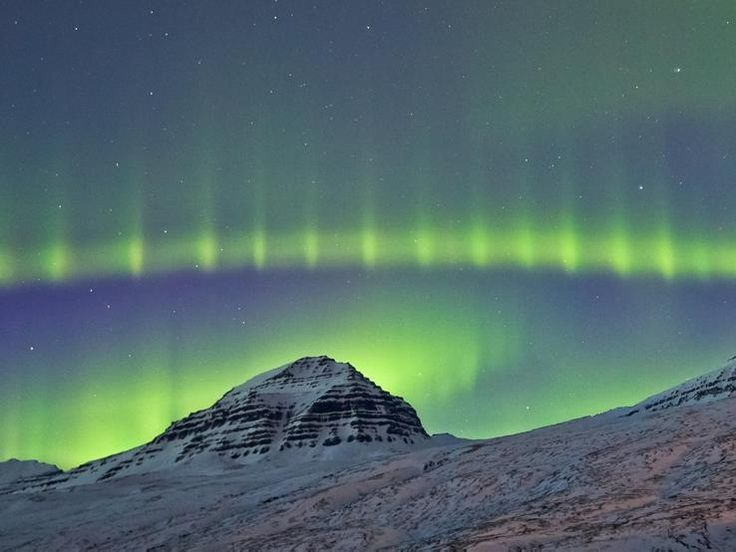
\includegraphics[width=0.8\textwidth]{images/aurora1.jpg}
    \caption{Полярное сияние (Aurora Borealis)}
    \label{fig:aurora1}
\end{figure}

Тема важна не только из-за интереса к процессам между Солнцем и Землей, но и из-за практики. Авроральная активность --- заметный пример космической погоды. Сильные магнитные бури с яркими сияниями могут сбивать спутники, влиять на линии электропередач, трубопроводы в высоких широтах и мешать радиосвязи и GPS. Поэтому понимание механизмов сияний полезно и в науке, и на практике.

\textbf{Цель работы} --- собрать и систематизировать физику возникновения полярных сияний, описать их виды и факторы, которые влияют на них.

Для достижения цели нужно:
\begin{enumerate}
    \item Проследить, как менялись представления о полярных сияниях с древности до наших дней.
    \item Рассмотреть главные физические процессы: пересоединение магнитных линий, ускорение частиц и возбуждение газов атмосферы.
    \item Классифицировать виды сияний и связать их внешний вид с условиями их появления.
    \item На основе литературы оценить, какие направления в исследованиях перспективны, а какие нет.
\end{enumerate}

Объект исследования --- полярные сияния как природное явление. Предмет --- физика их возникновения, виды и влияющие факторы.

% Глава 1
\section{Историческая эволюция представлений о полярных сияниях}

\subsection{Древние наблюдения и донаучные гипотезы}

Первые записи о сияниях нашли в китайских хрониках около 2600 года до н.э., где описывали «красные облака в ночном небе». В Древней Греции Аристотель предположил, что сияния --- это огонь от испарений в верхних слоях атмосферы. Хотя эта теория оказалась ошибочной, сам поиск объяснений был важным шагом.

В мифах разных народов сияния имели разное объяснение. В скандинавских легендах это свет от щитов валькирий, финны ассоциировали с искрами от бегающей лисы, а русские называли сияния «пазорами» или «сполохами» и связывали с предзнаменованиями бедствий.

\subsection{Первые научные теории (XVII--XIX вв.)}

С XVII--XVIII веков ситуация изменилась. Галилей наблюдал сияние у Флоренции в 1621 году и дал ему имя «aurora borealis» --- северное сияние. В середине XVIII века российский учёный Франц Эпинус предположил электрическую природу сияний и связь с движением заряженных частиц~\cite{epinus1758}. Американец Бенджамин Франклин независимо выдвинул похожую гипотезу.

\subsection{Эксперименты К. Биркеланда и теория К. Стормера}

Серьёзный прорыв сделал норвежец Кристиан Биркеланд в конце XIX --- начале XX века~\cite{birkeland1908}. Он предположил, что сияния вызывают электроны от Солнца, которые идут к полюсам под влиянием земного магнитного поля. В лаборатории он поставил опыт с магнитным шаром и электронным пучком --- свечение появлялось только возле «полюсов» шара, как и в природе.

В 1930--1950-х Карл Стормер разработал теорию движения заряженных частиц в магнитном поле Земли~\cite{stormer1955}. Он показал, что электроны и протоны могут проникать в атмосферу только около полюсов.

\subsection{Формирование современной парадигмы: открытие солнечного ветра и магнитосферы}

Настоящая теория сформировалась в 1950--1960-х с запуском космических аппаратов. Выяснилось, что Солнце постоянно испускает плазму --- солнечный ветер. В 1961 году Джеймс Данжи предложил модель пересоединения магнитных линий~\cite{dungey1961}. Эта модель стала основой современной науки о полярных сияниях.

\begin{figure}[H]
    \centering
    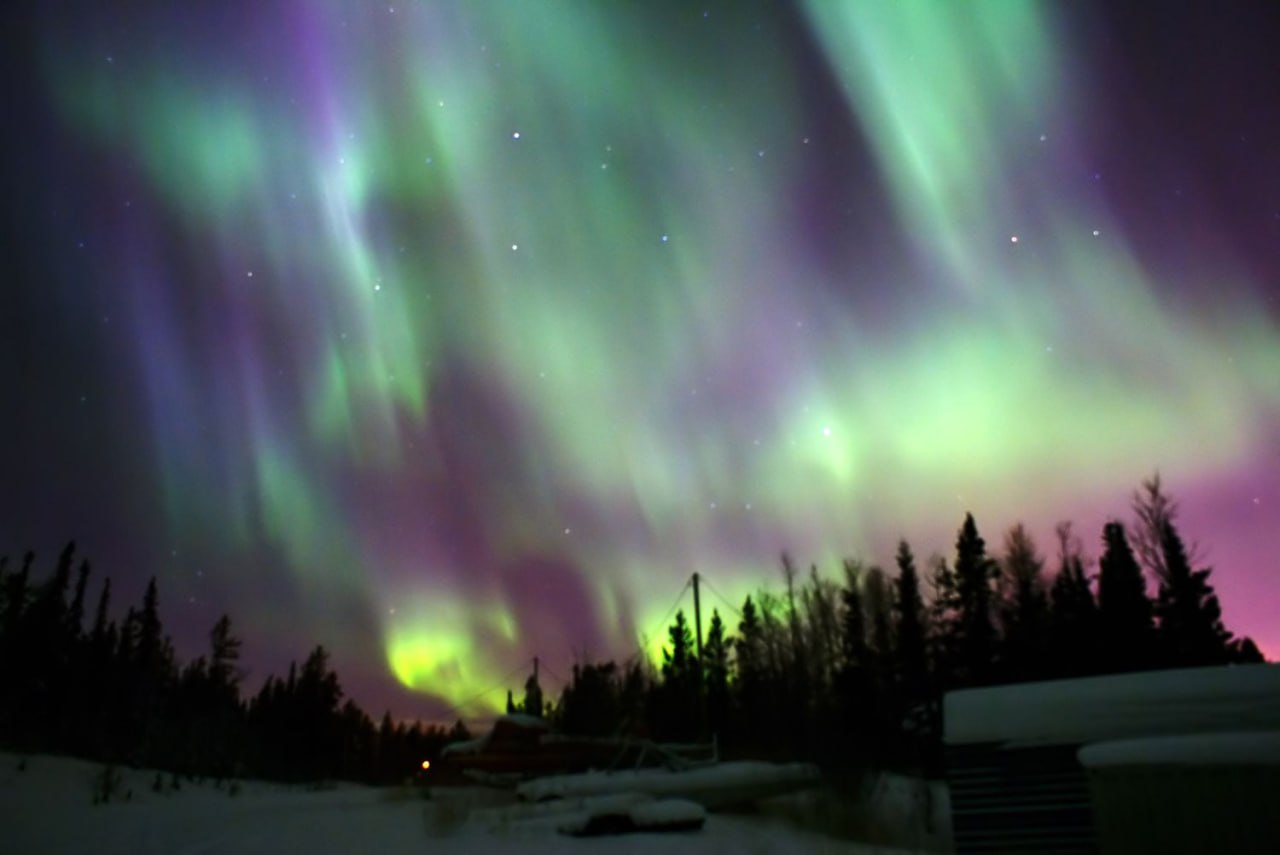
\includegraphics[width=0.8\textwidth]{images/aurora2.jpg}
    \caption{Дискретное полярное сияние (дуги и лучи)}
    \label{fig:aurora2}
\end{figure}

% Глава 2
\section{Физические механизмы возникновения полярных сияний}

\subsection{Солнечный ветер и межпланетное магнитное поле}

Солнечный ветер --- это поток плазмы из короны Солнца со скоростью 300--800 км/с. На орбите Земли плотность частиц составляет примерно 5--10 см$^{-3}$, температура достигает $10^5$--$10^6$ К. В состав входят электроны, протоны и немного альфа-частиц~\cite{kivelson1995}.

В солнечном ветре «заморожено» межпланетное магнитное поле (IMF) с напряжённостью около 5 нТл. Для взаимодействия с магнитосферой важна южная компонента $B_z$. При $B_z < 0$ создаются условия для пересоединения магнитных линий и усиления сияний.

\subsection{Пересоединение магнитных полей как первичный механизм}

Пересоединение --- процесс разрыва и соединения магнитных линий с изменением их топологии. В магнитосфере Земли он отвечает за передачу энергии от солнечного ветра во внутренние области~\cite{dungey1961}. Энергия, выделяемая при пересоединении, оценивается как:

\begin{equation}
    E_{\text{rec}} = \frac{B^2}{2\mu_0} \cdot V \cdot t,
    \label{eq:energy}
\end{equation}

где $B$ --- напряжённость магнитного поля, $\mu_0$ --- магнитная постоянная, $V$ --- объём области пересоединения, $t$ --- характерное время.

\subsection{Ускорение авроральных электронов}

Существует два основных механизма ускорения электронов до энергий 1--100 кэВ~\cite{lyons1984}.

\subsubsection{Квазистатическое ускорение}

Вдоль магнитных линий могут существовать стационарные электрические поля с напряжением 1--10 кВ. Электроны разгоняются в таких полях, приобретая энергию:

\begin{equation}
    E_e = e \cdot U,
    \label{eq:energy_electron}
\end{equation}

где $e$ --- элементарный заряд, $U$ --- разность потенциалов.

\subsubsection{Альфвеновское ускорение}

Альфвеновские волны --- колебания плазмы вдоль магнитных линий, которые также могут ускорять электроны без постоянного электрического поля. Скорость альфвеновских волн определяется формулой:

\begin{equation}
    v_A = \frac{B}{\sqrt{\mu_0 \rho}},
    \label{eq:alfven}
\end{equation}

где $\rho$ --- плотность плазмы.

Данные спутников THEMIS, Cluster и MMS показывают, что оба механизма работают одновременно~\cite{angelopoulos2008, burch2016}.

\subsection{Возбуждение атмосферных газов и интерпретация спектров}

Ускоренные электроны сталкиваются с атомами кислорода и азота, возбуждая их. Основные эмиссионные линии:
\begin{itemize}
    \item 557,7 нм (зелёная) --- кислород, высоты 100--120 км;
    \item 630,0 нм (красная) --- кислород, высоты 200--300 км;
    \item 391,4 и 427,8 нм (синие/фиолетовые) --- молекулярный азот, ниже 100 км.
\end{itemize}

% Глава 3
\section{Типология полярных сияний и определяющие факторы}

\subsection{Диффузное и дискретное сияние}

Выделяют два главных типа полярных сияний по форме и физическим механизмам (см. табл.~\ref{tab:types}).

\begin{table}[H]
    \centering
    \caption{Сравнение диффузного и дискретного сияний}
    \label{tab:types}
    \begin{tabular}{|p{4cm}|p{5cm}|p{5cm}|}
        \hline
        \textbf{Характеристика} & \textbf{Диффузное сияние} & \textbf{Дискретное сияние} \\
        \hline
        Форма & Равномерное свечение & Чёткие структуры (дуги, лучи) \\
        \hline
        Размер & Сотни километров & 1--10 км \\
        \hline
        Длительность & Несколько минут & Секунды \\
        \hline
        Механизм ускорения & Альфвеновский & Квазистатический \\
        \hline
    \end{tabular}
\end{table}

\subsection{Зависимость цвета от высоты и энергии частиц}

Цвет свечения зависит от состава атмосферы и энергии электронов:
\begin{itemize}
    \item Электроны $\sim$1 кэВ вызывают красное свечение ($\lambda = 630$ нм) на высоте $\sim200$ км.
    \item Электроны 5--10 кэВ создают зелёное свечение ($\lambda = 557,7$ нм) на высоте 100--120 км.
    \item Электроны $>$30 кэВ проникают ниже 100 км и вызывают синие и фиолетовые оттенки ($\lambda = 391,4$ нм и $427,8$ нм).
\end{itemize}

\subsection{Внешние факторы}

Интенсивность и частота полярных сияний зависят от:
\begin{enumerate}
    \item \textbf{11-летнего солнечного цикла:} в максимуме активности сияния ярче и чаще.
    \item \textbf{Геомагнитной активности (индекс Kp):} при Kp $\ge$ 5 наблюдаются бури, сияния видны в средних широтах.
    \item \textbf{Сезона:} максимум активности приходится на март и сентябрь (равноденствия).
\end{enumerate}

% Глава 4
\section{Методы наблюдения и моделирования}

\subsection{Наземные инструменты}

Наземные наблюдения включают авроральные камеры, фотометры, радары некогерентного рассеяния (EISCAT) и магнитометры. Сети камер, такие как THEMIS Ground Network, отслеживают движение сияний в реальном времени.

\subsection{Космические миссии}

Космические аппараты позволяют измерять процессы в магнитосфере:
\begin{itemize}
    \item \textbf{THEMIS} (NASA, 2007) --- пять спутников, локализовавших точку старта суббури~\cite{angelopoulos2008}.
    \item \textbf{Cluster} (ESA, 2000) --- четыре спутника для изучения трёхмерных структур.
    \item \textbf{MMS} (NASA, 2015) --- высокое временное разрешение для изучения пересоединения~\cite{burch2016}.
\end{itemize}

\subsection{Программная реализация моделирования движения частиц}

Ниже представлен фрагмент программного кода на Python, моделирующий движение заряженной частицы в магнитном поле Земли методом Бориса.

\begin{minted}[frame=lines, framesep=2mm, fontsize=\small, linenos]{python}
import numpy as np
import matplotlib.pyplot as plt

"""
Моделирование движения заряженной частицы в магнитном поле Земли
(метод Бориса для уравнения движения в магнитном поле)
"""

def boris_step(r, v, B, q, m, dt):
    """
    Один шаг метода Бориса для движения частицы в магнитном поле.
    
    Параметры:
        r - позиция (x, y, z)
        v - скорость (vx, vy, vz)
        B - магнитное поле в точке r
        q - заряд частицы
        m - масса частицы
        dt - шаг по времени
    """
    # Полу-шаг для скорости
    v_minus = v + 0.5 * dt * (q / m) * np.cross(v, B)
    
    # Поворот в магнитном поле
    t = (q * dt * 0.5 / m) * B
    s = 2 * t / (1 + np.dot(t, t))
    v_prime = v_minus + np.cross(v_minus, t)
    v_plus = v_minus + np.cross(v_prime, s)
    
    # Полный шаг
    v_new = v_plus + 0.5 * dt * (q / m) * np.cross(v_plus, B)
    r_new = r + v_new * dt
    return r_new, v_new

# Параметры частицы (электрон)
q = -1.602e-19      # заряд, Кл
m = 9.109e-31       # масса, кг
v0 = np.array([1e6, 0, 0])   # начальная скорость, м/с
r0 = np.array([6.4e6, 0, 0]) # начальная позиция, м
dt = 1e-5           # шаг, с
n_steps = 10000     # количество шагов

# Массивы для траектории
r_traj = [r0.copy()]
v_traj = [v0.copy()]

# Основной цикл
r = r0.copy()
v = v0.copy()
for _ in range(n_steps):
    # Простейшая модель дипольного поля
    R = np.linalg.norm(r)
    B = np.array([0, 0, 1e-5 * (6.4e6 / R)**3])  # Bz только для примера
    r, v = boris_step(r, v, B, q, m, dt)
    r_traj.append(r.copy())
    v_traj.append(v.copy())

print(f"Моделирование завершено. Количество шагов: {n_steps}")
\end{minted}

\subsection{Математическое моделирование}

Три основных подхода: глобальные MHD-модели (LFM, BATSRUS), кинетические модели (трассировка частиц) и гибридные модели (MHD + кинетика). Прогнозы авроральной активности достигают около 70\% точности.

% Глава 5
\section{Методы наблюдения и моделирования}

\subsection{Наземные инструменты}

Наземные наблюдения включают авроральные камеры, фотометры, радары некогерентного рассеяния (EISCAT) и магнитометры. Сети камер, такие как THEMIS Ground Network, отслеживают движение сияний в реальном времени.

\subsection{Космические миссии}

Космические аппараты позволяют измерять процессы в магнитосфере:
\begin{itemize}
    \item \textbf{THEMIS} (NASA, 2007) --- пять спутников, локализовавших точку старта суббури~\cite{angelopoulos2008}.
    \item \textbf{Cluster} (ESA, 2000) --- четыре спутника для изучения трёхмерных структур.
    \item \textbf{MMS} (NASA, 2015) --- высокое временное разрешение для изучения пересоединения~\cite{burch2016}.
\end{itemize}

\subsection{Программная реализация моделирования движения частиц}

Ниже представлен фрагмент программного кода на Python, моделирующий движение заряженной частицы в магнитном поле Земли методом Бориса.

\begin{minted}[frame=lines, framesep=2mm, fontsize=\small, linenos]{python}
import numpy as np
import matplotlib.pyplot as plt

"""
Моделирование движения заряженной частицы в магнитном поле Земли
(метод Бориса для уравнения движения в магнитном поле)
"""

def boris_step(r, v, B, q, m, dt):
    """
    Один шаг метода Бориса для движения частицы в магнитном поле.
    
    Параметры:
        r - позиция (x, y, z)
        v - скорость (vx, vy, vz)
        B - магнитное поле в точке r
        q - заряд частицы
        m - масса частицы
        dt - шаг по времени
    """
    # Полу-шаг для скорости
    v_minus = v + 0.5 * dt * (q / m) * np.cross(v, B)
    
    # Поворот в магнитном поле
    t = (q * dt * 0.5 / m) * B
    s = 2 * t / (1 + np.dot(t, t))
    v_prime = v_minus + np.cross(v_minus, t)
    v_plus = v_minus + np.cross(v_prime, s)
    
    # Полный шаг
    v_new = v_plus + 0.5 * dt * (q / m) * np.cross(v_plus, B)
    r_new = r + v_new * dt
    return r_new, v_new

# Параметры частицы (электрон)
q = -1.602e-19      # заряд, Кл
m = 9.109e-31       # масса, кг
v0 = np.array([1e6, 0, 0])   # начальная скорость, м/с
r0 = np.array([6.4e6, 0, 0]) # начальная позиция, м
dt = 1e-5           # шаг, с
n_steps = 10000     # количество шагов

# Массивы для траектории
r_traj = [r0.copy()]
v_traj = [v0.copy()]

# Основной цикл
r = r0.copy()
v = v0.copy()
for _ in range(n_steps):
    # Простейшая модель дипольного поля
    R = np.linalg.norm(r)
    B = np.array([0, 0, 1e-5 * (6.4e6 / R)**3])  # Bz только для примера
    r, v = boris_step(r, v, B, q, m, dt)
    r_traj.append(r.copy())
    v_traj.append(v.copy())

print(f"Моделирование завершено. Количество шагов: {n_steps}")
\end{minted}

\subsection{Математическое моделирование}

Три основных подхода: глобальные MHD-модели (LFM, BATSRUS), кинетические модели (трассировка частиц) и гибридные модели (MHD + кинетика). Прогнозы авроральной активности достигают около 70\% точности.

% Заключение
\section*{Заключение}
\addcontentsline{toc}{section}{Заключение}

В данной работе достигнута цель --- систематизированы физические механизмы полярных сияний, их типы и определяющие факторы.

Основные выводы:

\begin{enumerate}
    \item \textbf{Физика сияний} включает три ключевых этапа: пересоединение магнитных линий на границе магнитосферы, ускорение электронов (квазистатическое и альфвеновское), возбуждение атомов атмосферы с излучением фотонов.
    
    \item \textbf{Типы сияний} делятся на диффузные (равномерное свечение, альфвеновское ускорение) и дискретные (дуги, лучи, корона, квазистатическое ускорение). Цвет зависит от высоты и энергии частиц: красный ($\sim$200 км), зелёный (100--120 км), синий/фиолетовый (ниже 100 км).
    
    \item \textbf{Внешние факторы}: южная компонента IMF ($B_z<0$), скорость солнечного ветра, индекс Kp, фаза солнечного цикла (максимум), сезон (равноденствия).
    
    \item \textbf{Методы изучения}: наземные приборы (камеры, радары, магнитометры), космические миссии (THEMIS, Cluster, MMS, Swarm) и численные модели (MHD, кинетические, гибридные).
    
    \item \textbf{Перспективные направления}: гибридные модели, использование сияний для мониторинга атмосферы, машинное обучение. Неперспективны: поиск единого механизма ускорения, чистая статистика без физики, простое увеличение разрешения спутников.
\end{enumerate}

Полярные сияния перестали быть загадкой. Они стали важным индикатором космической погоды, что необходимо для безопасности спутников, линий электропередач и связи в высоких широтах~\cite{kivelson1995, pasachoff2013}.

% Список литературы
\bibliographystyle{ugost2003}
\bibliography{thesis}

\end{document}